\chapter{Analyse}
\label{ch:Analyse}
%TODO Problem analysieren, Verwendbare Topologien aussuchen, 

\section{Verwandte Arbeiten - Selbstlokalisierung \& indirekte Fernlokalisierung mit 802.11}
%TODO Einleitung

\subsection{WiFi-LLS}
\label{ch:Vorherige:sec:LLS}
Chen et al. stellen mit dem WiFi-based Local Location System (WiFi-LLS) ein System zur indirekten Fernlokalisierung vor \cite{chen2007design}.
Als Messgröße wird die Stärke des empfangenen Signals (received signal strength, RSS) genutzt. 
Diese wird laut 802.11 Spezifikation als Index (RSSI) von der Hardware zurückgegeben. \\
Für die Ortung wird zunächst der RSSI von Paketen naher Access Points gemessen und zusammen mit der MAC-Adresse der mobilen Einheit in ein Paket gepackt und an den Ortungsserver versendet.
Anschließend wird auf dem Ortungsserver ein theoretisches Signalausbreitungsmodell $P(d) = P(d_0) - 10log_{10}(\frac{d}{d_0})^n - OAF$ mit der Distanz $d$, der Signalstärke $P(d)$ und der Referenzdistanz $d_0 = 1$m zur Bestimmung der Position der mobilen Einheit verwendet. \\
$P(d_0)$, der Pfadverlustexponent $n$ und der Hindernisdämpfungsfaktor $OAF$ müssen bestimmt werden, jedoch lassen sich $P(d_0)$ und $n$ auf einer einzelnen Teststrecke mit unterschiedlichen Abständen von AP und mobiler Einheit bestimmen. $OAF$ kann sogar für einen Gebäudetyp einmalig bestimmt werden.
Dadurch hat das Modell einen konstanten Aufwand. 
Dies ist für Baustellen interessant, da sich diese Werte einmalig messen und dann sogar über mehrere gleichartige Baustellen übertragen ließen.\\
In dieser Veröffentlichung steht die Ortungsgenauigkeit im Vordergrund und es werden keine Angaben zum Energieverbrauch gemacht. 
Als Referenz kann dienen, dass die mobile Einheit bei WiFi-LLS alle 5 Sekunden einen Scan (siehe Abschnitt \ref{ch:phase1:sec:scan}) durchführt, dann werden die Signalstärken entdeckter APs zusammen mit der eigenen MAC-Adresse in XML codiert und das so erzeugte Paket an den Ortungsserver versendet.

\subsection{AiRISTA Flow RTLS}
Ekahau bietet unter der Marke \textit{AiRISTA Flow RTLS} eine zu WiFi-LLS ähnliche Lösung kommerziell an \cite{airista2017airista}.
Ihr Ekahau B4 Badge Tag ermittelt regelmäßig den RSSI zu nahegelegenen APs und versendet diese an einen Ortungsserver \cite{liu2007survey}.
Das Tag bietet darüber hinaus noch einige Zusatzfunktionen, so können über die Datenverbindung auch Nachrichten und Alarmierungen an das Tag gesendet werden und die drei angebrachten Knöpfe können programmiert werden.\\
Bezüglich des Energieverbrauchs gibt sich das Informationsblatt des B4 Badge Tag vage: Das Tag soll abhängig vom Ortungsintervall wochenlang halten, danach muss der $600\ mA/h$ Akku geladen werden \cite{ekahau2017b4}.
Das Informationsblatt zum Ekahau W4, welches statt um den Hals am Handgelenk getragen wird, gibt an, dass der verbaute $530\ mA/h$ Akku bei einem Ortungsintervall von 15 Sekunden 500 Stunden (ca. 21 Tage) hält \cite{ekahau2017w4}.\\
AiRISTA Flow spricht auf ihrer Website zum Beispiel Krankenhäuser, Schulen und Regierungseinrichtungen an, hier sollen zusätzlich bewegliche Objekte, wie etwa Krankenhausbetten, geortet werden.
Die dazu verwendeten Asset Tags werden über einen Beschleunigungssensor aktiviert und können, wenn die Objekte selten bewegt werden, deutlich längere Laufzeiten erreichen \cite{ekahau2017a4}. \\

\subsection{AeroScout}
Auch das AeroScout System von Stanley Healthcare richtet sich an den medizinischen Sektor und soll Objekte und Personen orten \cite{aeroscout2017asset}, \cite{aeroscout2017staff}.
Da sich auch dieses System in das bestehende WLAN-Netzwerk einfügt, sollte es ebenfalls auf einer indirekten Fernlokalisierung beruhen und demnach ähnliche Eigenschaften bezüglich des Energieverbrauchs aufweisen.\\
Das Informationsblatt ihres T14 Tags für Personen gibt eine Laufzeit von bis zu drei Wochen, abhängig von Konfiguration und Typ des Tags, an \cite{aeroscout2017t14}. 
Eine Angabe zu dem verwendeten Typ, der Konfiguration oder der Kapazität des verbauten Akkus wird nicht gemacht.\\

\subsection{Selbstlokalisierung mit Szenenanalyse}
\label{ch:Vorherige:sec:RSS-basierte}
Prasithsangaree et al. stellen ein System zur Selbstlokalisierung vor \cite{prasithsangaree2002indoor}, es verwendet aber eine offline-Phase zum Sammeln von Fingerabdrücken für Positionen in einem Abstand von 1,5 beziehungsweise 3 Metern. 
In diesen Fingerabdrücken werden die gemessenen RSSI der von den APs empfangenen Pakete als Merkmale zusammen mit der Position als Label gespeichert.
In der anschließenden online-Phase werden die gemessenen RSSI mit den Fingerabdrücken verglichen und die Position als gewichtetes Mittel der Labels bestimmt. \\
Die offline-Phase ist natürlich im Sinne der Aufgabenstellung nicht sinnvoll, da für eine Tunnelbreite von im Schnitt zehn Metern 4000 beziehungsweise 2000 Messungen pro Kilometer vorgenommen werden müssten.
Generell eignen sich Lösungen mit Szenenanalyse nicht gut für Baustellen, da diese nicht auf die potentiell höhere Genauigkeit angewiesen sind. 
Üblicherweise müssen dort sehr große Flächen vermessen werden und die Veränderungen durch den Baufortschritt führen dazu, dass regelmäßig neu gemessen werden muss.
Außerdem müssen bewegliche Störquellen wie Baumaschinen vorher aus dem Bereich entfernt werden, um unverfälschte Fingerabdrücke zu erhalten.
Der Aufwand ein System mit Szenenanalyse auf einer Baustelle zu betreiben ist deshalb sehr hoch und widerspricht der Forderung nach geringer Komplexität. \\
Die Arbeit zeigt aber die Volatilität der empfangenen Signalstärke auf, dies wurde 2011 von Lui et al. genauer untersucht \cite{lui2011differences}.
Lui et al. zeigen, dass die gemessene empfangene Signalstärke stark von der beteiligten Hardware abhängt und die Systeme jedes mal neu kalibriert werden müssen wenn sie auf ein neues AP-Modell portiert werden. 
Auf dem Areal sollte deshalb optimalerweise nur ein AP-Modell verwendet werden. \\
Abb. \ref{fig:luiRSSI} zeigt die gemessenen RSSI Werte für die von ihnen getesten Netzwerkkarten mit unterschiedlichen Distanzen, für einige Karten korreliert die empfangene Signalstärke nur sehr schwach mit der Distanz zwischen Knoten und mobiler Einheit.
Sie zeigen außerdem, dass einige AP-Modelle den RSSI speichern und nur bei größeren Veränderungen aktualisieren und dass die Antenne signifikanten Einfluss auf den protokollierten Wert hat.



\begin{figure}[h]
  \centering
	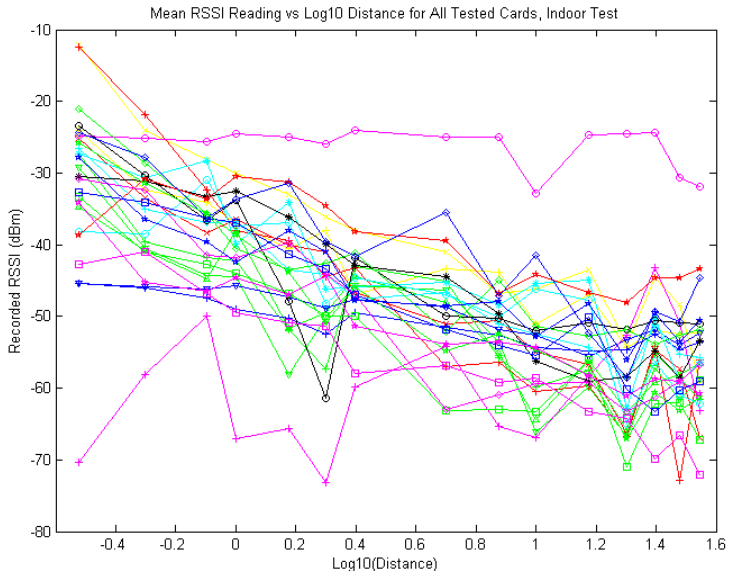
\includegraphics[width=\textwidth]{images/luiRSSI.png}
  \caption{Gemessener RSSI mit verschiedenen Access Points und Distanzen, aus \cite{lui2011differences}.}
  \label{fig:luiRSSI}
\end{figure}

\section{Verwandte Arbeiten - Fernlokalisierung \& indirekte Selbstlokalisierung mit 802.11}
%TODO Einleitung

\subsection{RADAR}
\label{ch:Vorherige:sec:RADAR}
Das RADAR System von Bahl et al. (Microsoft Research) hat als eins der ersten WLAN-basierten Ortungssysteme viel Aufmerksamkeit erfahren \cite{bahl2000radar}.
Als Messgröße wird die Stärke des empfangenen Signals (received signal strength, RSS) genutzt, diese wird laut 802.11 Spezifikation als Index (RSSI) von der Hardware zurückgegeben. 
Das RADAR System ist auf eine offline-Phase angewiesen, in der empirisch ein Signalausbreitungsmodell aufgebaut wird. 
Es handelt sich also um ein System mit Szenenanalyse.\\
Die Verwendung einer offline-Phase ist im stark veränderlichen Baustellenumfeld nicht akzeptabel. 
Zum einen führt der ständige Baufortschritt dazu, dass regelmäßig neu kalibriert werden muss und zum anderen wirken sich auch die großen Baumaschinen auf die Signalausbreitung aus. 
Damit sich dies nicht im Modell wiederfindet, müssten zunächst alle beweglichen Maschinen aus dem Bereich entfernt werden, um anschließend in der online-Phase ihren Einfluss glätten zu können.
Die offline-Phase ist deshalb wirtschaftlich gesehen nicht durchführbar und das empirisch ermittelte Signalausbreitungsmodell müsste durch ein theoretisches ersetzt werden, für eine grobkörnige Bereichsortung sollte dies jedoch ausreichend sein.\\
Bei RADAR sendet die mobile Einheit vier UDP-Pakete pro Sekunde aus, an den Knoten wird dann der RSSI gemessen.
Die Autoren weisen jedoch darauf hin, dass sich dieser Vorgang leicht umkehren ließe, um von einer Fernlokalisierung auf eine Selbstlokalisierung zu kommen.
Bezüglich des Energieverbrauchs äußern sie sich jedoch zu keiner der beiden Varianten.\\
Die Position wird anschließend bestimmt, indem aus den in der offline-Phase aufgenommenen Werten derjenige mit dem geringsten Abstand zu den gemessen Werten gewählt wird. 
Dies wird im \textit{nearest neighbour in signal space (NNSS)} Algorithmus beschrieben.
Für die Ortung wird mehrfach gemessen und dann gemittelt, um im Median eine Genauigkeit von unter 3 Metern zu erhalten. 
Das kurze Sendeintervall von 0,25 Sekunden führt auch bei bewegten Personen zu einer Genauigkeit von 3,5 Metern.
Gleichzeitig sorgt das kurze Sendeintervall aber auch für einem hohen Energieverbrauch auf Seiten der mobilen Einheit, eine Reduktion der Sendevorgänge sollte im Kontext der Bereichsortung angestrebt werden, um den Energieverbrauch zu senken und die Batterielaufzeit der mobilen Einheit zu steigern.

\subsection{Verbesserungen an RADAR}
Bahl et al. veröffentlichten anschließend noch einige Verbesserungen für das ursprüngliche RADAR System \cite{bahl2000enhancements}.
Diese umfassen unter anderem den Einsatz von Access Points statt PCs als Knoten, verbesserte Ortung bewegter Personen und die Erkennung von hinzugekommenen Hindernissen wie etwa Personen.
Letzteres geschieht durch die Analyse der Signalstärke von Beacons anderer APs, da diese sich nicht bewegen, können Veränderungen in der Signalstärke als Veränderungen auf dem Signalweg gesehen werden.
Dies ließe sich auch auf größere Hindernisse übertragen, hängt aber stark von der strategischen Platzierung und möglichst dichten Verteilung der APs ab.\\
Auch hier äußern sich die Autoren nicht zum Energieverbrauch, wohl auch deshalb weil sie einen Laptop als mobile Einheit verwenden.

\subsection{Time-of-flight Lokalisierung}
\label{ch:Vorherige:sec:TOF}
Aufgrund der Schwächen von RSS-basierten Systemen wurde auch über solche nachgedacht, die stattdessen oder zusätzlich die time-of-flight (TOF) messen. 
Ein Beispiel für ein solches zeigen Wibowo et al. \cite{wibowo2009time}. 
Sie fordern optimalerweise Zugriff auf die physische Schicht (PHY) des 802.11 Protokolls, da auf diesen aber üblicherweise kein Zugriff besteht, messen sie TOF in der darüber liegenden MAC-Schicht.\\
Ein Knoten sendet einen Beacon aus und protokolliert die Sendezeit, die mobile Einheit empfängt den Beacon, protokolliert die Empfangszeit und die Sendezeit der gesendeten Antwort, der Knoten sichert die Empfangszeit der Antwort.
Nun sendet die mobile Einheit die zwei gespeicherten Zeitstempel an den Knoten, der mit diesen die Verarbeitungszeit auf der mobilen Einheit berechnen kann, um dann die Distanz $d = c * (\frac{t_{empfangen} - t_{gesendet} - t_{Verarbeitung}}{2})$ zur mobilen Einheit zu bestimmen.
Dieses Schema lässt sich leicht von einer Fernlokalisierung in eine Selbstlokalisierung umwandeln, indem man den Initiator des Vorgangs tauscht.\\
Die Notwendigkeit die Zeitstempel bereits in der PHY- beziehungsweise MAC-Schicht zu setzen erfordert Zugriff auf die Software des als Knoten verwendeten Access Points. 
Außerdem müssen die Zeitstempel im Bereich von Nanosekunden gesetzt werden und die Verarbeitungszeit vor/nach dem Setzen muss sehr konstant sein, da eine Abweichung von 100 ns bei c = 299.792.458 m/s bereits einen Fehler von 30 Metern verursacht.\\
Muthukrishnan et al. beschreiben diese Problematik bei dem Versuch TOF ohne Zugriff auf die Software des APs umzusetzen \cite{muthukrishnan2006using}.
Sie kommen zu dem Ergebnis, dass sich die in der Spezifikation eingebauten Zeitstempelfunktionen wie das Network Time Protocol (NTP), Ping und die Zeitstempel in Beacons nicht eignen, da sie zum einen nur eine Auflösung im Millisekundenbereich bieten und zum anderen von der Blockierungskontrolle von 802.11 (CSMA/CA) abhängen.

\subsection{Ortung ohne mobile Einheit}
Eine Ortung ohne mobile Einheit erfüllt wegen ihrer Abwesenheit offensichtlich jede Anforderung an die Batterielaufzeit der mobilen Einheit.
Mit MonoPHY stellen Abdel-Nasser et al. ein System zur Ortung ohne mobile Einheit vor \cite{abdel2013monophy}. \\
Dazu verwenden sie einen 802.11n-fähigen Laptop und Access Point und analysieren die Channel State Information (CSI) der physischen Schicht (PHY) der zwischen AP und Laptop übertragenen Daten.
Um die bestehende Struktur von APs zu nutzen, sollte das System angepasst und die CSI zwischen den APs gemessen werden.
Es hat jedoch einige Aspekte, die es ungeeignet für die Aufgabenstellung machen.\\
Das System unterscheidet nicht zwischen Personen, sondern erkennt nur, dass jemand anwesend ist. 
Außerdem ist es nur für eine Person in einem 100 $m^2$ Apartment gestaltet worden und müsste auf Baustellengröße und die Verfolgung vieler Personen erweitert werden.
Aber auch dann ist fraglich, wie gesichert werden kann, dass alle Personen durchgehend erkannt werden können, zum Beispiel wenn sich mehrere Personen auf oder in einem Transportfahrzeug aufhalten.
Auch ist es ohne Identifikation schwerer Fehler zu erkennen. 
Wird fälschlicherweise angezeigt, dass sich noch eine Peron im Tunnel befindet, kann oft durch ausrufen des Betreffenden festgestellt werden, dass dieser nicht im Tunnel ist. 
Hat man dagegen nur die Information, dass sich noch eine Person im Tunnel befindet, hat man keine Möglichkeit schnell herauszufinden ob dies der Wahrheit entspricht.\\
Weitere Probleme entstehen durch die Baumaschinen und Container. 
Diese haben einen starken Einfluss auf die CSI und verdecken dadurch möglicherweise nahe Personen und die Fahrzeugführer.
Deshalb müssten diese Objekte ebenfalls als Entitäten angezeigt werden. 
Die Anzeige diverser Kommandostände, Pausenräume und stehen gelassener Baumaschinen verwirrt im Notfall jedoch, da sich in jedem Objekt potentiell eine Person befinden könnte.\\
Die Veröffentlichung beruht außerdem auf der Verfügbarkeit der CSI, diese sind dort durch die Auswahl einer bestimmten Netzwerkkarte gegeben und sind nicht zwingend in einer bestehenden Struktur von APs verfügbar.
Als letzter Kritikpunkt steht die Verwendung eine offline-Phase, die, wie bereits diskutiert, wirtschaftlich nicht umsetzbar ist. \\ 
Somit erfüllt die Ortung ohne mobile Einheit zwar die Anforderungen an den Energieverbrauch, jedoch nicht die Forderung nach sicherer Erkennung von Abschnittswechseln, deshalb scheidet diese Technik zumindestens für Baustellen aus.

\section{Verwandte Arbeiten - Funkbasierte Lokalisierung ohne 802.11}
%TODO Einleitung

\subsection{Geeignete Messwerte für Bluetooth}
Hossain et al. untersuchen die laut Bluetooth Spezifikation zurückgegebenen Messwerte bezüglich ihrer Eignung für die Lokalisierung \cite{hossain2007comprehensive}.\\ 
Link Quality (LQ) beschreibt, wie gut die Verbindung zwischen zwei Geräten ist.
Der Wert wird aus der Bitfehlerrate beim Empfänger berechnet, allerdings ist nicht spezifiziert, wie der Wert zu berechnen ist, er hängt also in hohem Maße vom Hersteller des Empfängers ab. \\
Der Received Signal Strength Indicator (RSSI) misst die Stärke des eingehenden Signals, die Spezifikation sieht jedoch eine Golden Receive Power Range (GRPR) vor. 
Liegt der RSSI über oder unter dieser wird eine Anfrage zum erhöhen oder verringern der Sendeleistung an das andere Gerät verschickt, dies dient während einer aktiven Verbindung dazu den Energieverbrauch zu senken.
Problematisch am RSSI ist, dass er relativ zur GRPR bestimmt wird.
In der Untersuchung von Hossain et al. führte das dazu, dass der RSSI mit 0 gemessen wurde, wenn er innerhalb der GRPR lag. \\
Transmission Power Level (TPL) ist die Sendeleistung eines Geräts. 
TPL kann während einer bestehenden Verbindung durch Anfragen des Verbindungspartners verändert werden.
Dazu muss diese Energiesparfunktion jedoch unterstützt werden, was bei dem von Hossain et al. vwrwendeten Gerät nicht der Fall war.
Abb. \ref{fig:bluetoothmess} zeigt deshalb für TPL eine waagerechte Linie.\\
Für Inquirys wird die Stärke des eingehenden Signals ohne die Beactung des GRPR bestimmt.
Außerdem werden Inquirys immer mit voller Sendeleistung gesendet, da sie zur Entdeckung von Ressourcen verwendet werden.
Es handelt sich ebenfalls um den RSSI, um jedoch den Unterschied zum RSSI für eine Verbindung deutlich zu machen nennen Hossain et al. diesen Wert RX Power Level.

\begin{figure}[h]
  \centering
	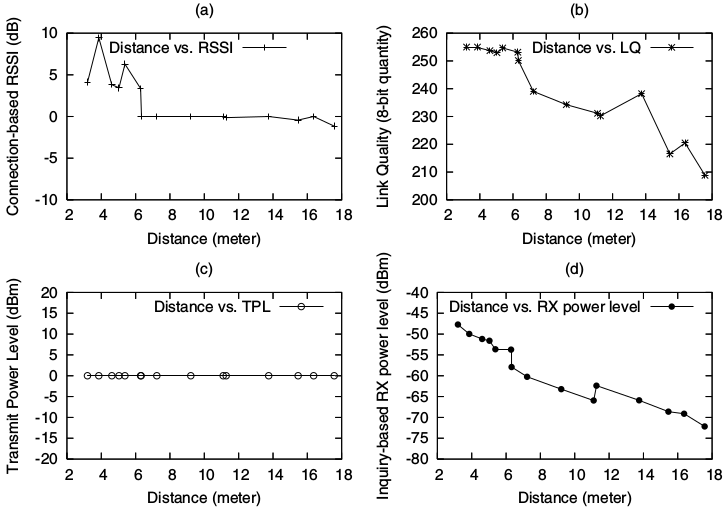
\includegraphics[width=\textwidth]{images/bluetoothmess.png}
  \caption{Korrelation der Messwerte mit der Distanz, aus \cite{hossain2007comprehensive}}
  \label{fig:bluetoothmess}
\end{figure}

\subsection{RSSI-basierte BLE Ortung}
Jianyong et al. stellen ein System zur Ortung auf Basis von Bluetooth Low Energie (BLE, auch Bluetooth Smart) vor \cite{jianyong2014rssi}. \\
Sie messen an den Knoten den RSSI von Inquirys, die zuvor von den mobilen Einheiten versendet wurden.
Für die genaue Ortung werden die Ergebnisse mit einem Gauß-Filter geglättet und für jeden Knoten die Parameter für ein Signalausbreitungsmodell bestimmt.
Das gemessene Signalstärke $P = A - 10n*log(d)$ hängt von der Referenzsignalstärke A im Abstand von einem Meter, dem Dämpfungsfaktor n und der Distanz d ab. \\
Jianyong et al. bestimmen die Referenzsignalstärke und den Dämpfungsfaktor für jeden Knoten.
Da jedoch nur eine Bereichsortung für diese Arbeit gefordert wurde, sollten A und n nur beispielhaft für einen Knoten bestimmt werden, um den Aufwand beim Aufbau der Infrastruktur zu reduzieren.
Abb. \ref{fig:blemodel} zeigt die von Jianyong et al. bestimmten Parameter für das Signalausbreitungsmodell. 
Abb. \ref{fig:blemodel} zeigt außerdem, dass die verwendeten CC2540 Development Kit von Texas Instruments von einem Access Point nur auf 20 Meter detektiert werden konnte.

\begin{figure}[h]
  \centering
	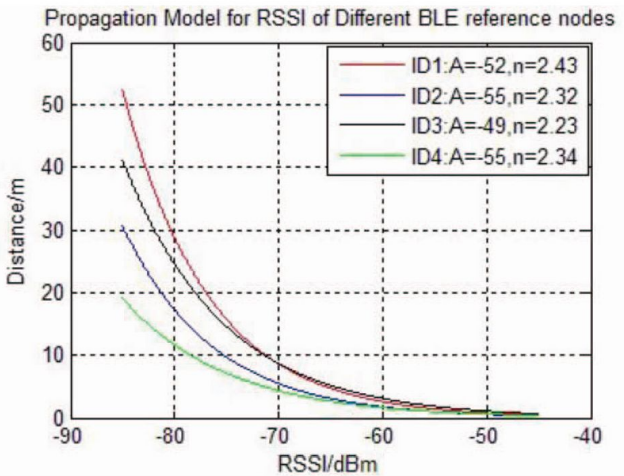
\includegraphics[width=0.7\textwidth]{images/blemodel.png}
  \caption{Signalausbreitungsmodelle aus \cite{jianyong2014rssi}}
  \label{fig:blemodel}
\end{figure}
